\chapter{The Material Layering Model}\label{cha:partsOfLayeredShader}

The next chapters focus exclusively on pattern based material layering systems and shaders. Therefore, material layering will always refer to pattern layering if not further specified. For the purpose of this work I developed a theoretical and implementation independent schematic model to describe material layering systems and shaders, the \emph{Material Layering Model}. This material layering model is inspired by the high level material layering systems form \emph{UE4} \ref{sec:matLayV2} and \emph{The Coalition} \cite{colin2017GearsOfWar}. It splits layered materials in different encapsulated components that are responsible for specific tasks. The main components of this material layering model are: \emph{Material Container}, \emph{Masking Container} and \emph{Blending Module} (see figure \ref{fig:patternBasedMaterialModel}). 

\begin{description}
	\item[Material Container:]
		The material container is an independent component in the material layering model. It represents an encapsulated module that uses different input data and outputs a material layer object.\footnote{The material layer object is a data type that describes the standardized material properties by defining the individual channel values influencing the corresponding render passes.} The computations taking place within this component can be complex but do not influence the other components of the material layering model. Like a class in programming, the implementation can change without effecting other components as long as the inputs and outputs stay the same. For most of this work it is enough to interpret a material container as a blackbox that inputs different data, does some computation based on them and exports a material layer object. 
 
	\item[Masking Container:]
		The masking container is responsible for generating a 0 to 1 mask that defines the influence intensity and area of the blending module. The masking container can be seen as encapsulated module inputing arbitrary data and optional material layer inputs. The masking container specifies the needed inputs and the logic that is used to derive the 0 to 1 masking information. 
		
	\item[Blending Module:]
		The blending module is responsible for the actual blending process of the individual material containers. The blending module inputs the material layers from the material containers and the mask output from the Mask Container. The blending module outputs a new material layer. As mentioned before, the 0 to 1 output of the masking container defines the area and intensity in which the blending takes place. The blending module includes the information of how to blend the individual material layer channels. The material layer output of the blending module can represent the final Shader output, a new material container for further layering or an intermediate result for further manipulation within the shader. 
\end{description}

\begin{figure}
	\centering
	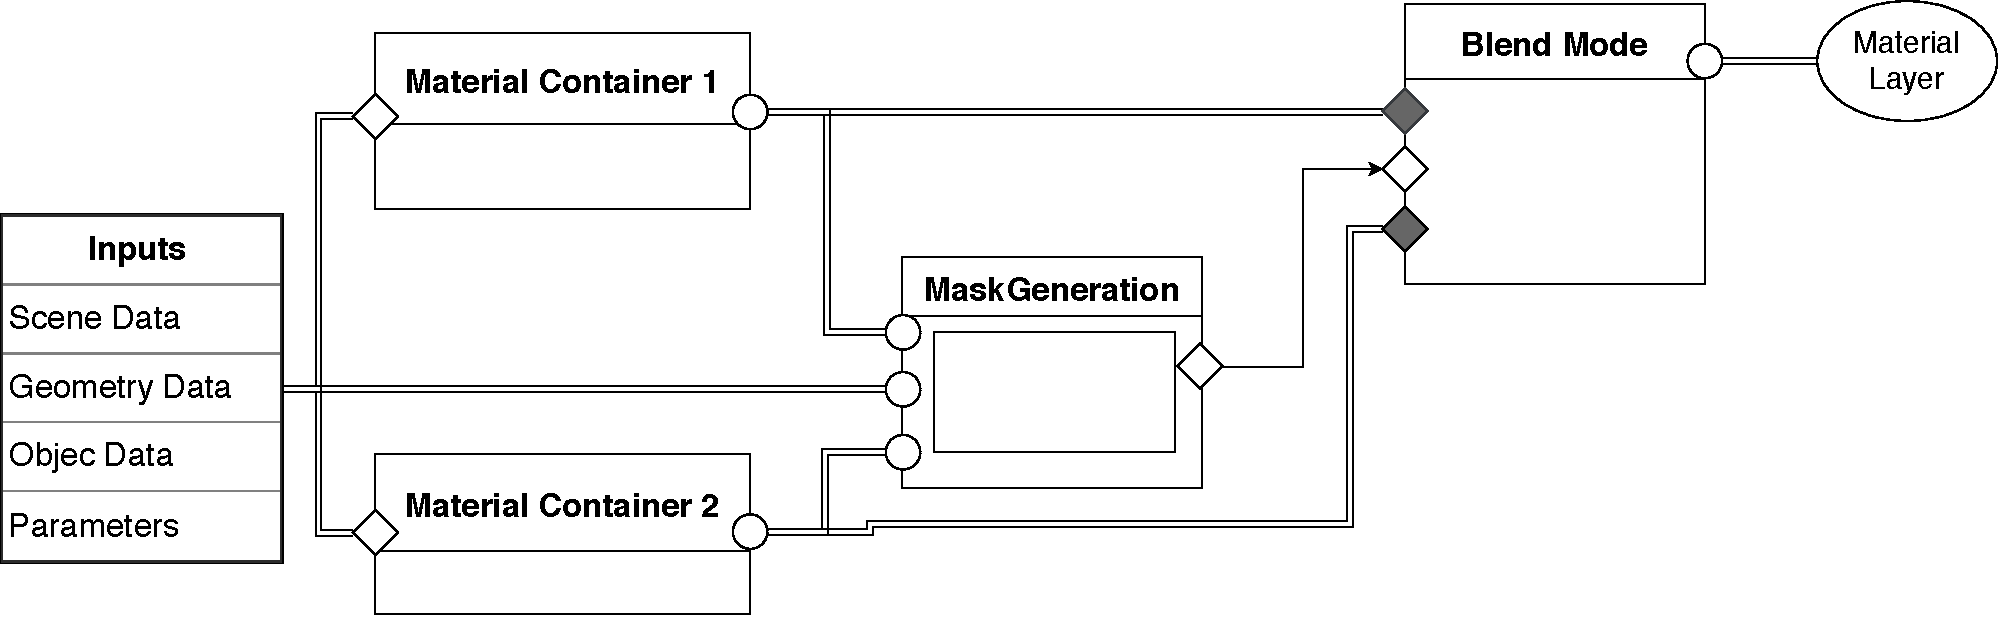
\includegraphics[width=0.95\linewidth]{images/04cha_01_LayeredMaterialComponents.pdf}
	\caption{Material Layering Model.}
	\label{fig:patternBasedMaterialModel}
\end{figure}

As already mentioned before, this is a theoretical and schematic model to establish a language that can be used for the design patterns in chapter \ref{cha:patterns}. It is intended to work for the different  material layering systems within this work. It does neither define how those systems are implemented on a technical level nor how material layering should be implemented. The material layering Model works for either describing a layered material shader or a layering system. In the former case, it represents the structure within the shader that enables the layering of different base materials. In the latter, it represents the structure of the system that is used to compute the final shader from the inputs. 

\begin{description}
	\item[Layered Material Shader:]
		The shader defines the amount of components (e.g., material containers) and the possible inputs. Adding additional inputs and options, changing or replacing individual components or modifying the blending behavior needs to be done manually on the shader level.  
	\item[Layered Material System:]
		Generally, the layered material system is implemented as a tool---normally within the engine---that uses different encapsulated modules, e.g., \emph{Material Layer} (material containers) and \emph{Material Layer Blends} (combining mask containers and blending module) in \emph{UE4}. These components can be combined easily within the tool. The layered material system does generate the shader code automatically in the background. Individual components can therefore be added, replaced or changed easily without any additional work.  
\end{description}





\section{Inputs}\label{sec:inputs}

	Inputs define which data is accessible from within the different modules of the material layering model. This section is mostly relevant for the material container and masking container components. These components have full access to all input data exposed by the engine: parameters, scene data, object data and mesh data. The material layering model does not define inputs as an independent sub module but as inherent part of the other modules. Which input data can be accessed from the shader is defined by the shading language, engine and tool that is used to create the shader. An overview of all  nodes and inputs for \emph{UE4} can be found in its documentation.\footnote{See the list of all nodes and inputs accessible from within the \emph{UE4} shader graph: \url{https://docs.unrealengine.com/en-us/Engine/Rendering/Materials/ExpressionReference}.} A huge amount of different data can be accessed, some of them are specific to special use cases. The following sections do not include all possible inputs but, in my opinion, the most useful and universal ones.  
	

	\subsection{Parameters}
	
		Parameters are variables that get exposed from within the shader or layering system. They can be set and modulated on a per material or component basis, depending on the implementation. This enables the user to create multiple distinctive materials using the same shader. These parameters can be global or specific to individual components. The available data types for parameters are defined by the shading system. The shader graphs of \emph{UE4} and \emph{Unity} support different data sets. All supported and predefined parameters available in \emph{UE4} shader graph can be found in the documentation.\footnote{See the documentation about parameter expressions: \url{https://docs.unrealengine.com/en-us/Engine/Rendering/Materials/ExpressionReference/Parameters}.} The most important ones are: textures, vectors, scalars and booleans.
		
		Textures are the most common way to store larger data sets for individual materials including color information, information about the lighting interaction, vectors, masking and many more. They are efficient in processing as they represent a simple data table than can be read and does not need heavy computation. Algorithms and workflows, like dynamic texture streaming, channel packing, mid mapping, compression and other optimizations make it possible to load a huge amount of bigger textures into a 3D scene. Nevertheless, the memory in the VRAM is limited and needs to be used carefully. Sending and managing the  data and render jobs to the GPU (draw calls) can lead to a bottleneck on the CPU. It is therefore important not to go overboard with the amount of textures and especially the texture resolutions. Vectors, scalars and booleans are incredible versatile and powerful as they can be used to define, drive and influence an infinite number of different operations. Vectors and scalars can be used to define and manipulate  colors, directions, normals, switches, remapping, intensities, rotations, vertex positions, uv coordinates etc. Most of the parameters can be changed and assigned at runtime. This works for all parameters that do not enforce the shader to recompile (e.g., static switches in \emph{UE4}).
	 	
	 
	\subsection{Scene Data}
	
		Different data from the 3D scene can be accessed in addition to the previously mentioned inputs. Some examples are are: mesh data using the corresponding material, data about the object owning the material and different arbitrary scene data exposed by the engine. Some examples for the latter are: data connected to cameras, lights, render passes. The separation between object and mesh related inputs is important as the usages for these data types are different. The mesh data is independent from the 3D scene. So for instance, object related values like hierarchy, position, rotation, scale do not have any influence on them. All of the identical meshes within the 3D scene share this data. All the material inputs are the same for those meshes. Object related inputs, on the other hand, are related to the position and hierarchy within the 3D scene. Therefore, inputs can be both influenced or independent from the mesh data. 
		
		\begin{description}
			\item [Mesh Related:] These inputs are only influenced by the mesh, e.g., UV coordinates, face and vertex normals, objects space position and object space normal. 	
			\item [Object Related:] In contrast to mesh related input, they may differ across objects even by using the identical mesh, e.g., world space normals, world space position, object position, rotation and scale. They can both be independent and influenced by the assigned mesh data. 
			\item [Scene Data:] Contains additional information of different objects within the scene like light vectors, camera position and distances to other objects. 
		\end{description}

	\subsection{Material Layer}

		The material layer is a data type that describes the standardized material properties by defining the individual channel values influencing the corresponding render passes. This standardized format makes it easy to blend and process base material information in a generalized way. This input can be used to drive procedural processes within the masking or material container. In the context of \emph{UE4}, this concept corresponds to \emph{Material Attributes}.\footnote{See the article about \emph{Material Attribute Expression} in the  \emph{UE4} documentation \url{https://docs.unrealengine.com/en-us/Engine/Rendering/Materials/ExpressionReference/MaterialAttributes}.} 
 
\section{Material Container}

	\begin{figure}
		\centering
		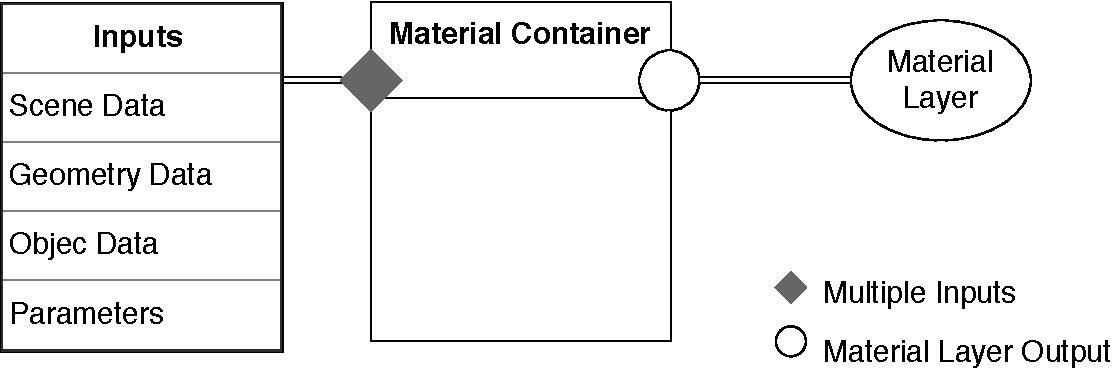
\includegraphics[width=0.75\linewidth]{images/04cha_02_LayeredMaterialComponents_materialContainer.pdf}
		\caption{Material Container.}
		\label{fig:MaterialContainer}
	\end{figure}


	This category describes the parts of the material layering system or shader graph that are used to define the surface properties of a base material. A material container is defined by different input data like textures, variables, mesh data, scene data or material layers and the computation happening within. The material container outputs a standardized material layer object. Figure \ref{fig:MaterialContainerSimpleComplex} shows two base materials: a simple and a complex one. A common workflow is to use textures to define the influence of the material on the individual rendering passes. This is a proven approach and used across many productions. The material container performs limited to no computation at all, except combining those textures to a material layer object and pass it on. Another approach is to use a more procedural workflow. In this case the material creation can react and adopt dynamically to different input data. This input data is used by procedural instructions. This can be a position and height based gradient tint or time based offset of the UV coordinates. The possibilities are limitless. As these instructions are usually calculated at runtime, they do not use a lot of memory but rely heavily on computations. Using parametric inputs in contrast to textures is usually a trade-off between memory and computation time.
	
	\begin{figure}
		\centering\small
		\begin{tabular}{@{}cc@{}}
			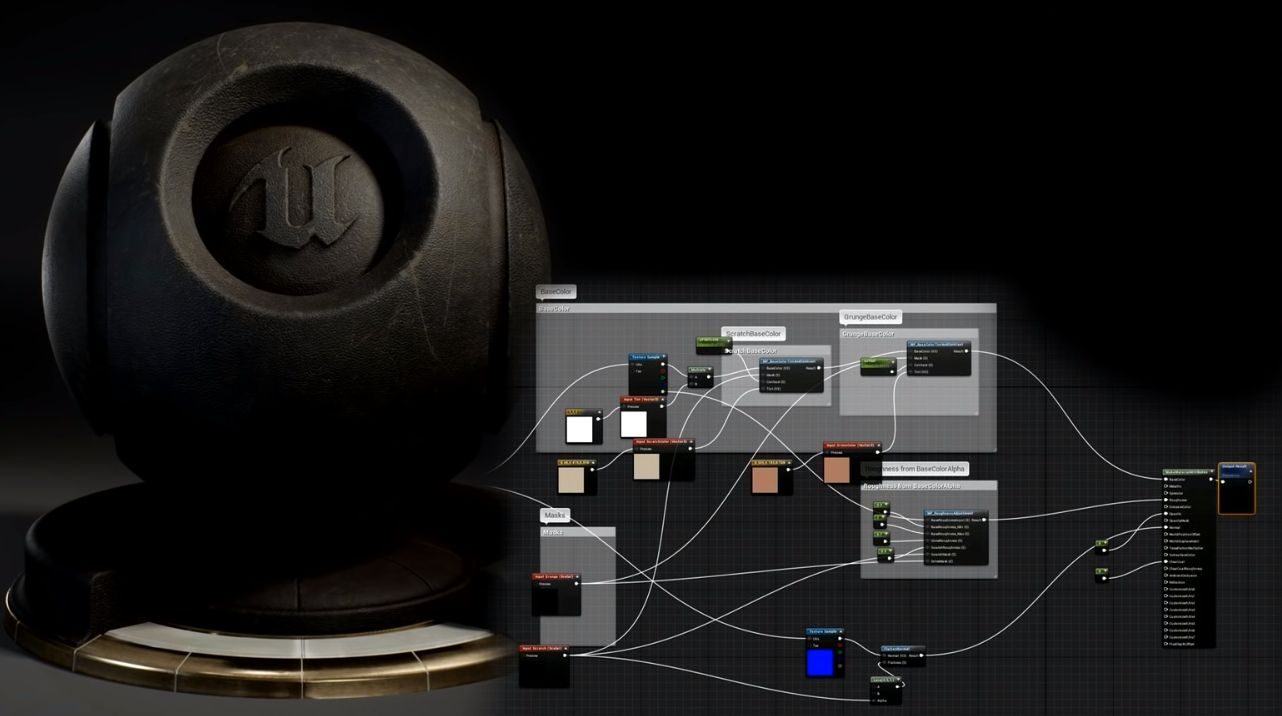
\includegraphics[width=0.475\textwidth]{04cha_03_paragonMat_simple.jpg} &		% JPEG file
			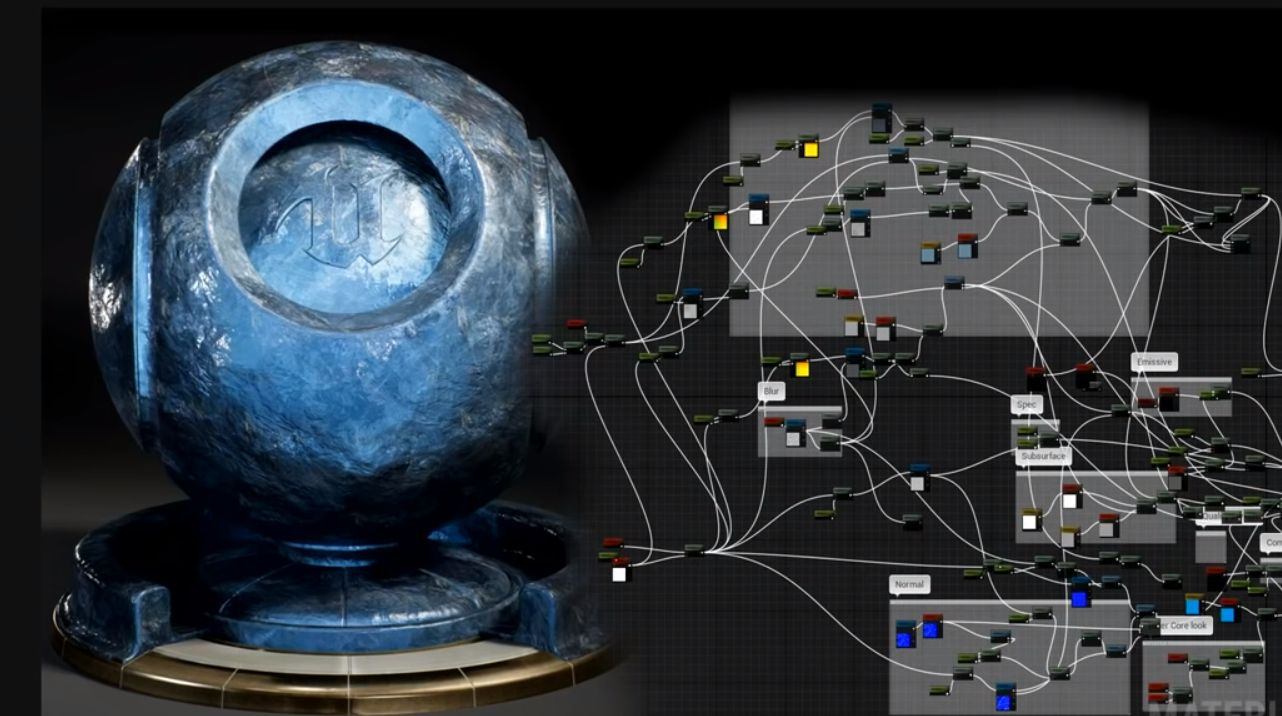
\includegraphics[width=0.475\textwidth]{04cha_03_paragonMat_complex.jpg} \\	% PNG file
			(a) & (b) 
		\end{tabular}
		\caption{Example of independent material containers in \emph{UE4}. These materials are implemented as material functions in \emph{UE4}. Both base materials use the same material parameter outputs but differ in complexity: (a) simple base material, (b) complex base material. Image source: \cite{moore2017pipeline}.}
		\label{fig:MaterialContainerSimpleComplex}
	\end{figure}	


\section{Masking Container}

	\begin{figure}
		\centering
		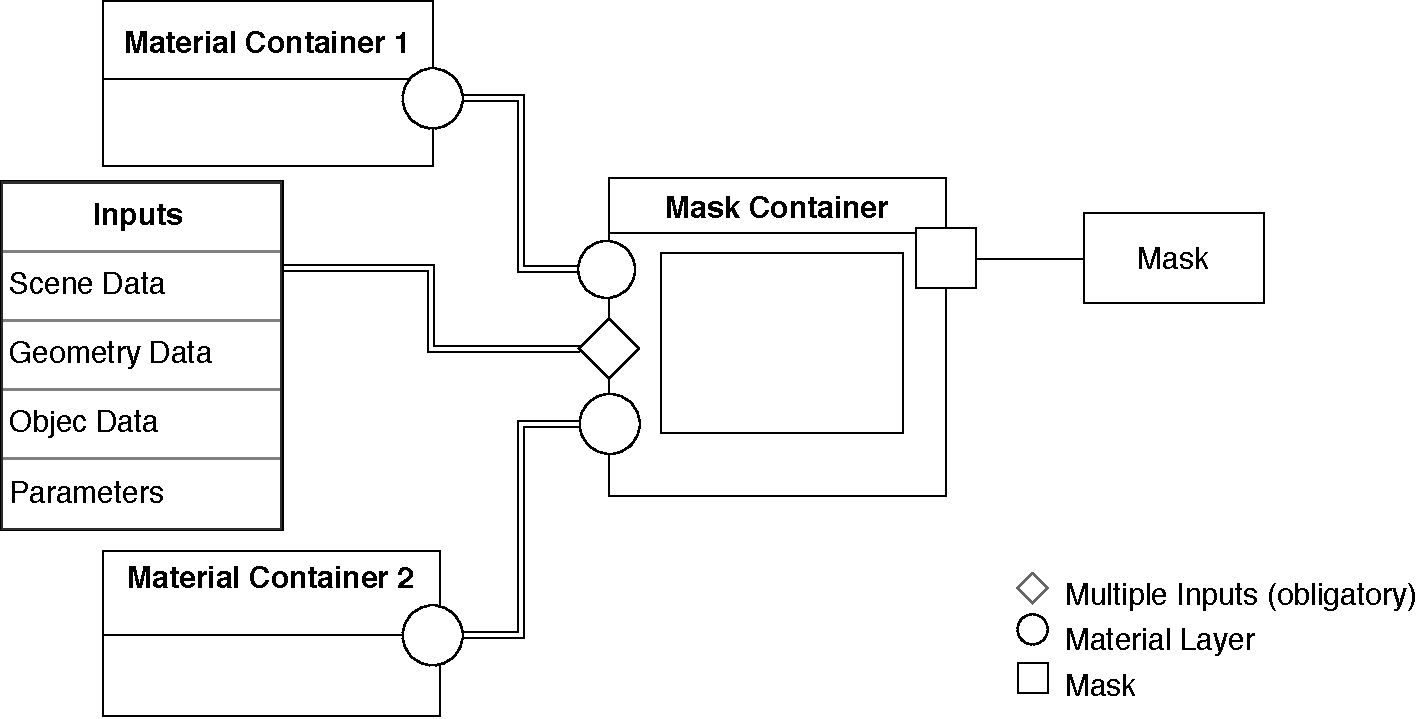
\includegraphics[width=0.75\linewidth]{images/04cha_04_LayeredMaterialComponent_MaskingContainer.pdf}
		\caption{Masking Container.}
		\label{fig:MaskingContainer}
	\end{figure}

	The masking container is responsible for controlling the affect area and intensity of the blending module. It provides the same full access to the different inputs as the material container. Nevertheless, texture masks are the most supported input type within material layering systems.  
	Texture masks are an intuitive and straight forward approach of masking out areas. The value 1 (white) means that the texture is visible while the value 0 (black) means it is not. The values in-between allow partial blending between the inputs and therefore allow to mix different values---in this case different material container within the blending module. 
	There are many different approaches to how to generate and project those masks onto a mesh. Some applications like \emph{Substance Painter}, \emph{DDO Painter}, \emph{Blender}, \emph{3D Coat}, \emph{Mari} allow to paint masks directly onto the mesh itself. This provides a lot of control over the actual blending. Procedural processes or baked maps can also be involved in the creation process of these texture masks.
	It is important to keep in mind that the final texel density does not dependent on texture mask resolutions. The texture resolution does only influence the resolution of the blending, i.e., the transition between the affected material components. The higher the mask resolution is the more detailed the transition between the textures appears. A 1k mask can be used to blend two 4k textures. This means that the object texel density is sixteen times higher than the texel density of the mask. For optimization and organization reasons gray scale masks are often stored in different color channels within one single texture. These textures are often called id maps. Each color channel (red, green, blue, alpha\footnote{The alpha channel is expensive in terms of memory consumption.  Using the alpha channel doubles the used memory for this texture as \emph{UE4} changes the compression format from DXT1 to DXT5 \cite{epic2015supportsettings}.}) represents another mask. The same rules as for the gray scale masks also apply to the ones within the color channels. An additional one can be stored within the alpha channel. Other commonly used inputs to influence the masking generation are vertex color, object and world position, object and wold space normal. Some of these inputs can be used to create different results even though the meshes are instantiated and shared. The different properties of these inputs can be used to achieve different behavior depending on the desired result.  
	
	The masking container can use and combine different inputs to compute the final mask output. Every input type has individual advantages and disadvantages. To get the most out of the blending, it is useful to combine different input types and combine texture based and procedural methods to generate the mask. Combining different inputs and methods can also be used to create additional detail for the main mask. This allows to either use methods that do not provide detailed masks (e.g., vertex color, world position, world space normals) or textures that have a low resolution. Additional details can be added later on by using additional inputs. An easy way to do so is to blend the main mask with a secondary tillable texture mask. This secondary mask is used to generate the small scale details. Using different blending modes (e.g., multiply, screen, add) gives a lot of control. Another less common approach is to use procedural noises as they are more expensive in terms of computation cost.
	
\section{Blending Module}\label{sec:blendingModule}

\begin{figure}
	\centering
	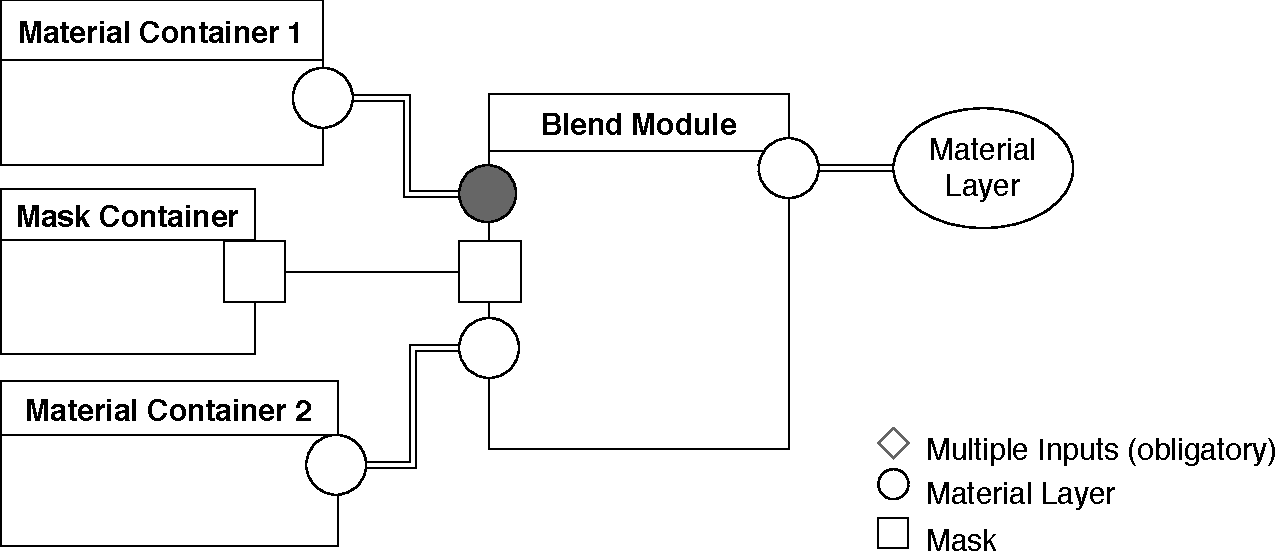
\includegraphics[width=0.75\linewidth]{images/04cha_05_LayeredMaterialComponents_BlendModule.pdf}
	\caption{Blending Module.}
	\label{fig:blendModule}
\end{figure}

The blending module describes the part of the material layering model that is responsible for the blending of the different base materials. There are many different ways to do so. As mentioned in section \ref{sec:patternLayering}, the blending of the individual material parameters is not trivial. The first part of this section describes some of the common issues that need to be taken into account when creating a layered material shader or using a material layering system. It discusses issues on an implementation level of blending individual parameters. The second part focuses more on a high level analysis of blending entire material containers.    

\subsection{Blending Individual Parameters}\label{sec:blendindIssuesLayering}

The blending of the different parameters can easily produce unintended values. One of these cases can appear by blending input parameters individually that affect the same material input. Pesare \cite{pesare2017material} provides a small example to further illustrate this point in his blogpost. By blending the colors \emph{A} and \emph{B} the average color should be achieved. Color \emph{A} is gray with the rgb values (0.4, 0.4, 0.4), a diffuse gain of 0.5 and a resulting final color output of (0.2, 0.2, 0.2). Color \emph{B} is a black with the rgb values (0, 0, 0), a color gain of 0 and resulting final color output of (0, 0, 0). The final color is hoped to be (0.1, 0.1, 0.1) as this is the average of the two final color outputs. What we get instead is a color with an rgb value of (0.2, 0.2, 0.2), a color gain of 0.25 and a final color output of (0.05, 0.05, 0.05)!  

Another issue appears if the input parameter influences the output lobe in a non linear way. This is a common issue across different parameters. Commonly used algorithms to compute the specular lobes like Beckmann, GGX and GTR do not have a linear behavior between input and the size of the specular output. Therefore, the input values are not intuitive without remapping. They cause unexpected results when blending shiny with rough materials \cite[p.\,7--10 and 14--15]{karis2013real}. This fact can easily be seen in figure \ref{fig:roughnessAccumulation}. In practice, this issue is often taken care of by a careful shader design withing the 3rd party applications. The Disney \emph{principled BRDF} and the physical shading models of \emph{UE4} introduce a remapped quadratic roughness value to provide an approximately linear 0 and 1 roughness propagation \cite[p.\,15]{burley2012physically}\cite{karis2013real}. 

\begin{figure}
	\centering\small
	\begin{tabular}{@{}cc@{}}
		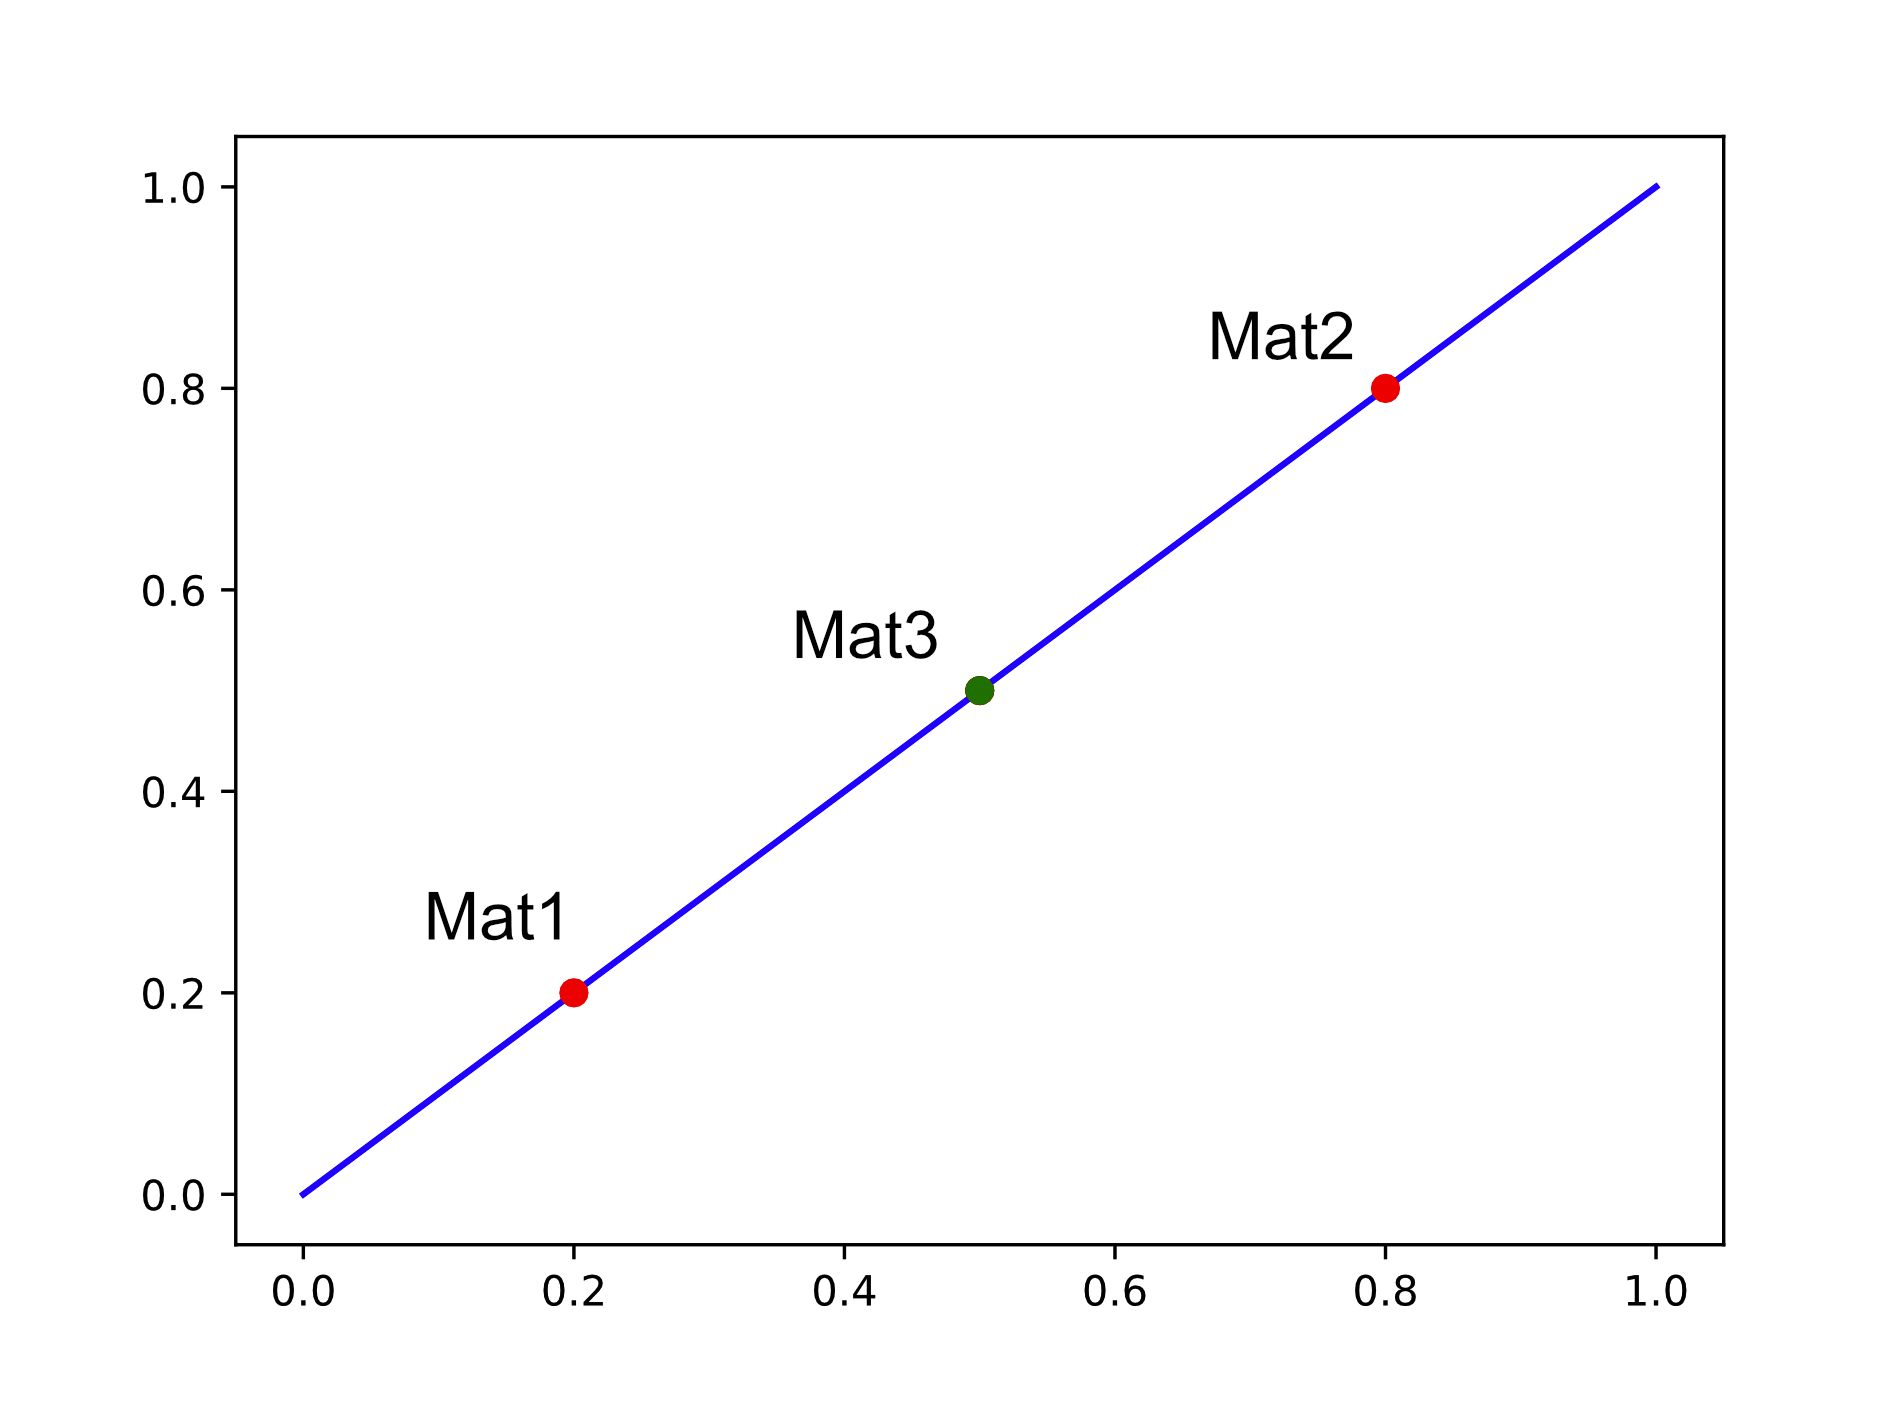
\includegraphics[width=0.475\textwidth]{04cha_06_linearRoughnessAccumulation.jpg} &		% JPEG file
		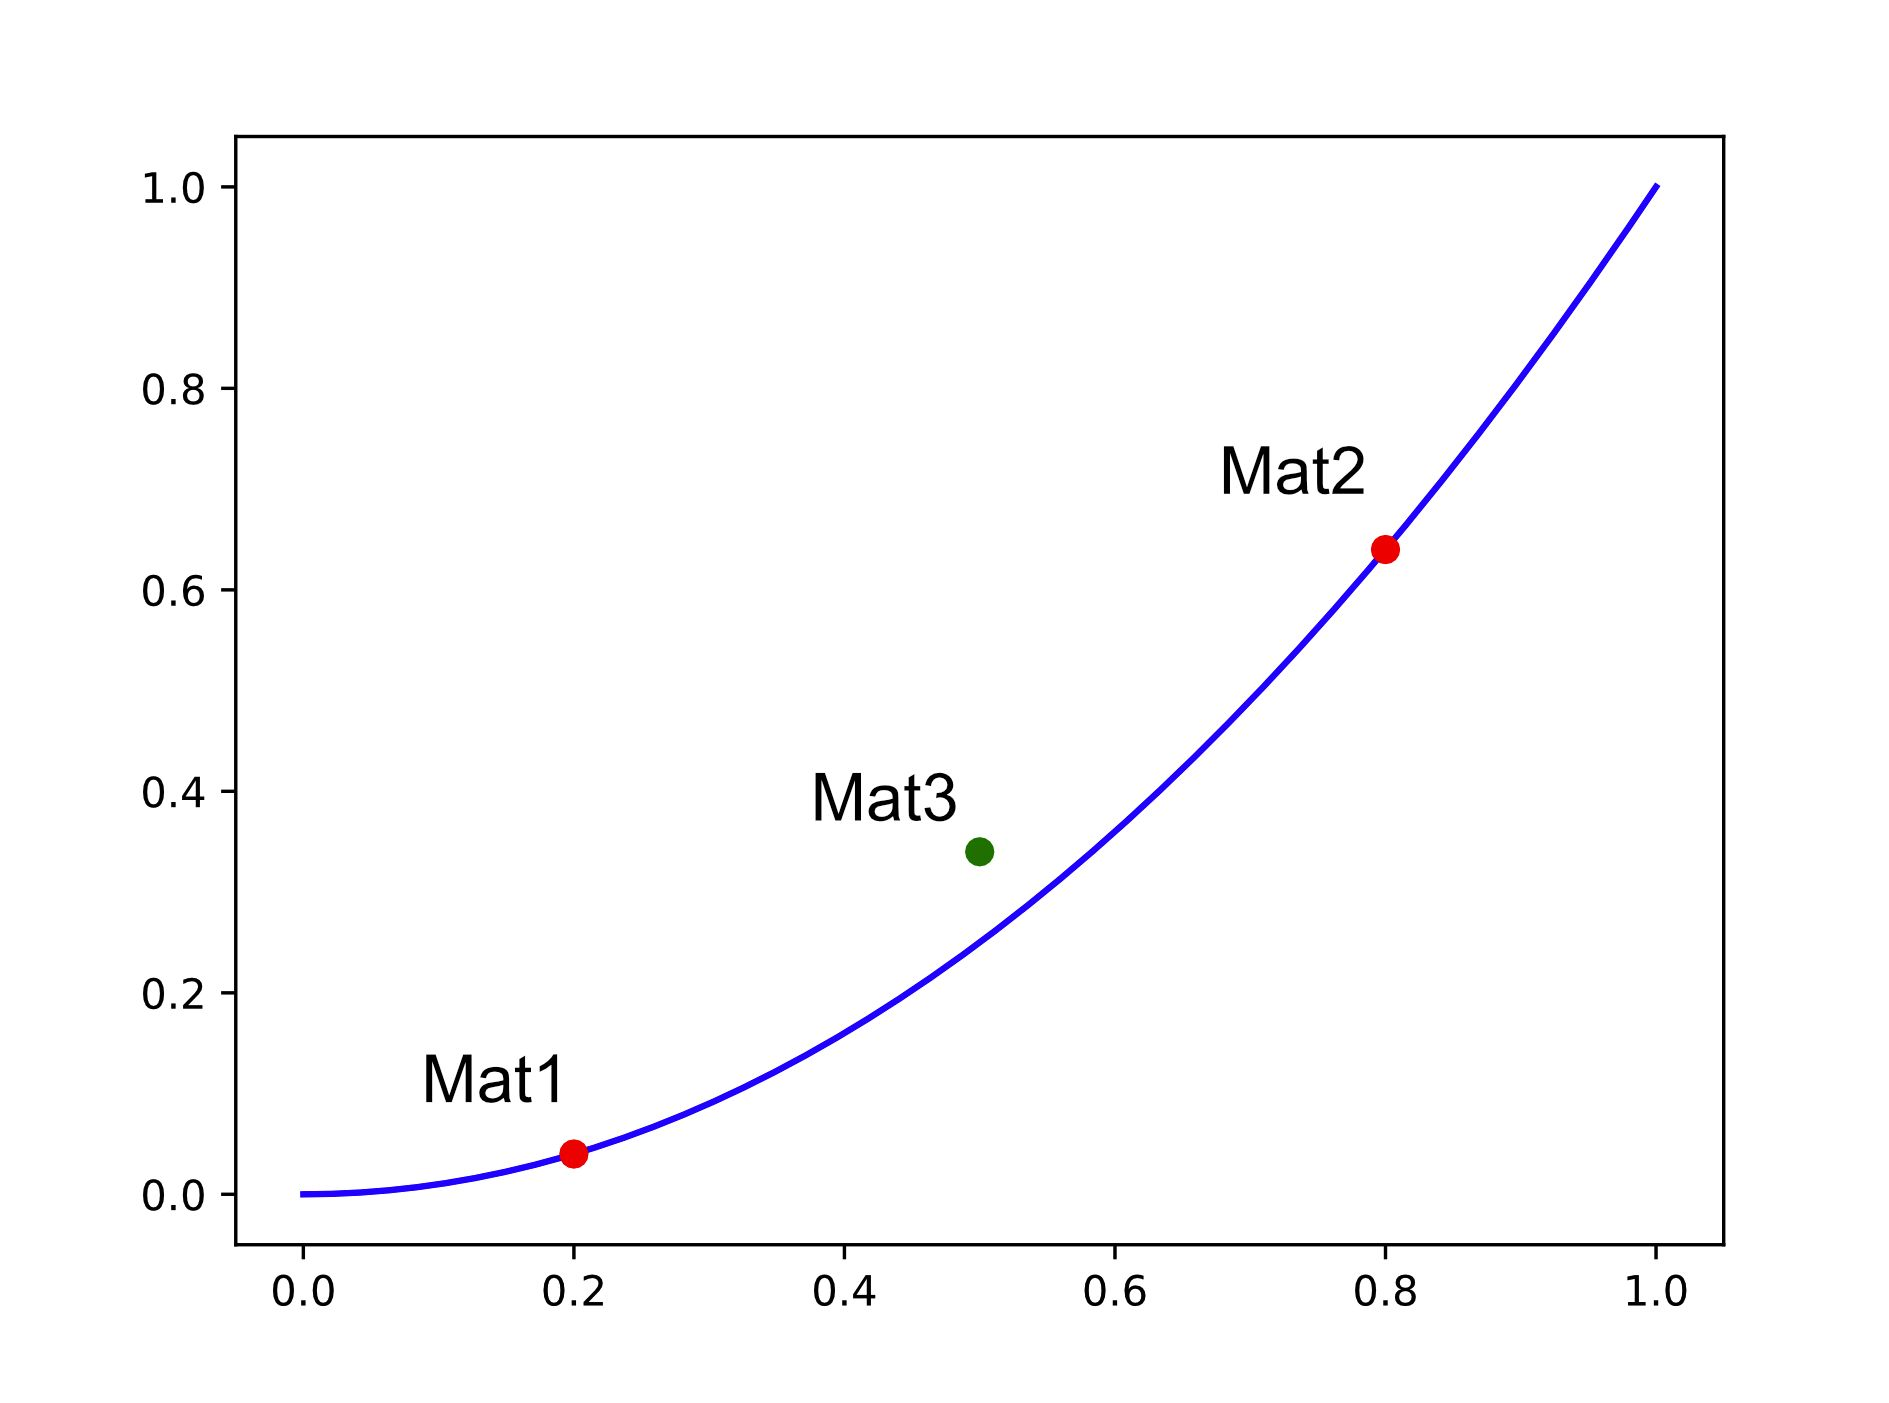
\includegraphics[width=0.475\textwidth]{04cha_06_exponentialRoughnessAccumulation.jpg} \\	% PNG file
		(a) & (b) 
	\end{tabular}
	

	\caption{Blending material properties with not linear value propagation. This can be caused by the algorithm or multiple values influencing the same output lobe. In figure (a) we can see that blending the inputs from \emph{Mat1} and \emph{Mat2} results in the expected output. In figure (b), on the other hand, the output result of linearly interpolating between value \emph{Mat1} and \emph{Mat2} results in a wrong value that is not on the output function. 
	}
	\label{fig:roughnessAccumulation}
\end{figure}


Another issue is the blending of two or more normal maps as they contain vector data. Simply adding or blending them does not bring the expected result. Jack Caron \cite{caron2014} does compare different approaches of blending normal maps on his website and provides some examples. To get a proper normal blending for the fire hydrant example in figure \ref{fig:approachesFireHydrant}, I used the approach proposed by  Christopher Dutton in \emph{Correctly and accurately combining normal maps in 3D Engines} \cite{dutton2013correctly}. There are many different types of data that need to be blended within a pattern layering system and every single one has to be treated differently. The effort to ensure a proper blending from an artist or tool's perspective is huge.


\subsection{Blending Modes}\label{sec:blendingModes}

The blending modes for physically based material layering are just a few. There are only a few possible ways how materials are combined in the real world. They are either mixed together, stacked on top of one another or transition from one material into an other. Recreating real world behavior is a common approach to build systems that work intuitively and consistently for the user. 
Weidlich \cite{weidlich2011thinking} explains that \emph{Weta Digital} uses a material layering system that tries to be highly physically accurate. The blending modes for the material layering system are based on real world examples. \emph{Weta Digital} includes two additional not physically plausible blending modes: one exclusively for adding emission and the other, rarely used one, for some specific exceptions. The following list contains the blending modes supported by the material layering system at \emph{Weta Digital}, which is an example for a physically plausible system \cite{weidlich2011thinking}: 

\begin{description}
	\item [Mix BxDFs:] Two substances are mixed and the physical properties get combined (e.g., ink in water).
	\item [Coating:] This method simulates the complex scattering process of light passing different thin material layers (e.g., water on ground, car paint).
	\item [Blending:] Blending allows a transition between different base materials.
	\item [Adding:] The adding of materials is only used for emissive materials as it breaks the energy conversation law and therefore is not physically plausible. Emissive materials break the energy conservation law anyway by introducing additional energy to the scene. It is therefore not relevant for them.
	\item [Subtract:] Subtract does not correspond to any physical plausible combination of materials and is only used in few special cases.
\end{description}

My first attempt to create layered materials for the project \emph{Letzte Worte} was to adopted this concept of using only a few physically plausible blending modes. During my research I found examples that use a much more flexible way of blending materials. In \emph{Paragon} \cite{paragon2016epic} they use the same normal maps for several base materials and blend only certain material properties to create material variation.
This shows that the demands to a blending module vary depending on its application. It makes sense to use limited physically plausable layer blending modes in the context of a highly physically based rendering process. Whereas giving the user more control over the blending process, allows for necessary performance optimization in high quality games. Texture count and computation times can be reduced by allowing custom blending modes with control over which material attributes are to blended and how. This represent a trade-off between accuracy, usability and performance. Some material containers in \emph{Paragon} are only described by a few parameters, instead of using a full material description on every material container. Instead of blending all material attributes, only the most important ones are blended. This decreases physically accuracy but increases performance dramatically. A powerful material layering system for real-time application should therefore include different options of how to define different materials and how to blend them. In the end, it is often a balancing act between physical accuracy, artistic freedom and performance.  Allowing the user to control if, how and which channels are supposed to be blended puts the power and responsibility into the hand of the user. It provides an active choice between performance,  usability and accuracy.

\emph{UE4} offers different nodes to blend material containers, override specific material layer attributes or get them individually. A list of these nodes can be seen in table \ref{table:layeredMaterialBlendTypes}. They take care of proper blending of individual parameters and therefore prevent users from tapping into issues correlated with pattern layering, discussed previously in section \ref{sec:blendindIssuesLayering}. It even offers different blending possibilities, e.g., the simple \emph{MaterialBlendNode} sacrifices accuracy for performance in comparison to the standard one.

\begin{table}
	\caption{Different Layered Material Blend Types in \emph{UE4}. Source: \cite{epic2015LayeredMats}.  }
	\label{table:layeredMaterialBlendTypes}
	\begin{longtable}{|p{3.5cm}|p{9.5cm}|}
		%\setlength\extrarowheight{2pt} % for a bit of visual "breathing space"
		\hline
		\small
		%\rowcolor{gray}
		Material Blend Mode                 &Description                                                                                                                                                                                                                                                                                                                                                \\ \hline
		AO 				  &Blends an ambient occlusion (AO) map over the surface to remove reflection.																					\\ \hline
		BaseColorOverride &Allows the Base Color to be replaced.                                                                                                                        \\ \hline
		BreakBaseColor    & Outputs the Base Color from an incoming Material Layer.                                                                                                       \\ \hline
		BreakNormal       & Outputs the Normal from an incoming Material Layer.                                                                                                          \\ \hline
		Decal             & Blends a decal sheet over the Material using the 2nd UV channel.                                                                                             \\ \hline
		Decal\_UV3        & Blends a decal sheet over the Material Layer using the 3rd UV channel.                                                                                       \\ \hline
		Emissive          & Blends an Emissive texture over the Material Layer.                                                                                                          \\ \hline
		GlobalNormal      & Blends a Normal texture over the Material Layer.                                                                                                             \\ \hline
		LightmassReplace  & Replaces the Base Color in Lightmass, allowing for changes to indirect lighting results.                                                                      \\ \hline
		ModulateRoughness & Multiplies the Material Layer's Roughness by an incoming texture. Useful for a ``greasy'' look.                                                               \\ \hline
		NormalBlend       & Blends a Normal texture across the surface, but by way of a mask texture, allowing for control of where the normal will appear.                              \\ \hline
		NormalFlatten     & Diminishes the effect of the Normal map.\,                                                                                                                     \\ \hline
		RoughnessOverride & Replaces the Roughness texture of a Material Layer.                                                                                                          \\ \hline
		Simple            & Provides a simple linear interpolation (Lerp) blending solution for 2 Material Layers. Does not blend Normal; instead, retains Normal of the Base Material.   \\ \hline
		Stain             & Blends the Top Material over the Base Material as a stain, meaning that only the Base Color and Roughness values from the Top Material are used.             \\ \hline
		Standard          & Blends all attributes of two Material Layers.                                                                                                                \\ \hline
		Tint              & Allows for tinting of a Material Layer by inputting a tint color and a mask to control the tint's location. Useful for making partial color changes.         \\ \hline
		TintAllChannels   & Similar to Tint, but also affects Specular. This is a very special case function; generally, you will not need it.                                           \\ \hline
		TopNormal         & Blends all attributes of both Materials but only uses the Normal of the Top Material.                                                                        \\ \hline
	\end{longtable}
\end{table}



\section{Summary}

In this chapter I introduced a schematic model to describe arbitrary material layering systems or shaders, the material layering model. It consist of three components: the material container, masking container and blending module. A material container has  arbitrary inputs defined in the shader or layering system and outputs a material layer object. The material layer object contains all information necessary to describe the rendering properties of a surface. The masking container can also access arbitrary inputs defined by shader or layering system. It outputs a 0 to 1 mask that is passed on to the blending module. The blending module is responsible for blending the material containers. The intensity and area of effect are defined by the mask.

Moreover, this chapter discussed shader inputs as they are an inherent part of both material container and masking container. To use and combine the distinctive properties of the individual inputs individually increases the possibilities of a material layering system. Finally, the blending modes and processes within the blending module were discussed. When blending material containers, the propagation, data type and input of individual parameters have to be considered. To simply interpolate linearly between different normal, roughness or ior values can produce unintended results. Another point to consider is how much control and freedom is given to the user. Should the blending module enforce accurate blending or concede the freedom to customize and optimize the blending process. The next chapter will put these abstract concepts into practice and will focus on the implementation of material layering methods into \emph{Unity} and \emph{UE4}.

